\begin{figure}[t]
\centering

\includegraphics[width=\columnwidth]{figures/fig5_baseline_bar_legend.pdf}
\begin{subfigure}{0.49\linewidth}
	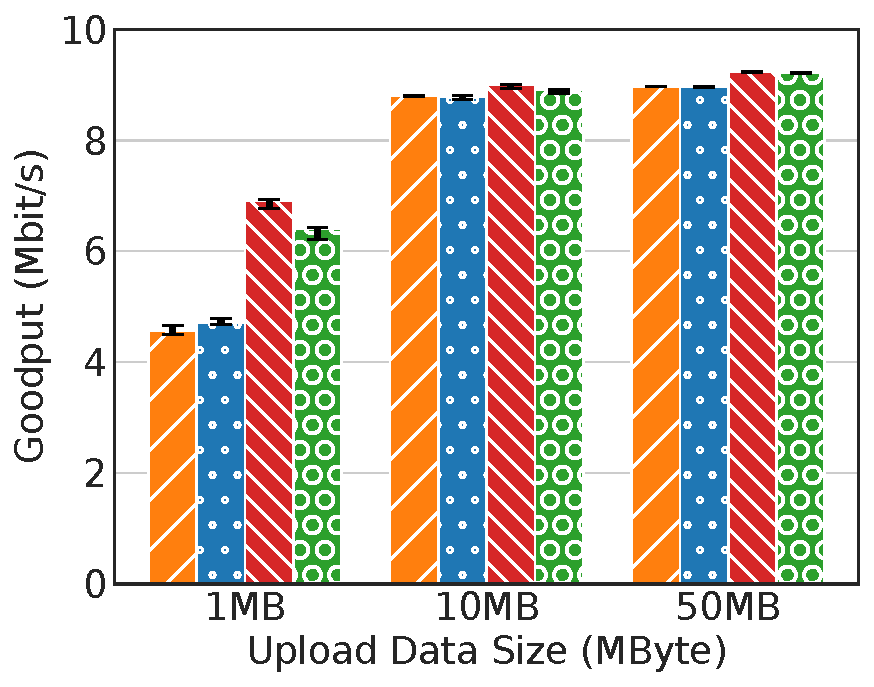
\includegraphics[width=\linewidth]{figures/fig5_baseline_loss0p.pdf}
	\caption{0\% loss.}
	\label{fig:baseline-bar:loss0p}
\end{subfigure}
\begin{subfigure}{0.49\linewidth}
	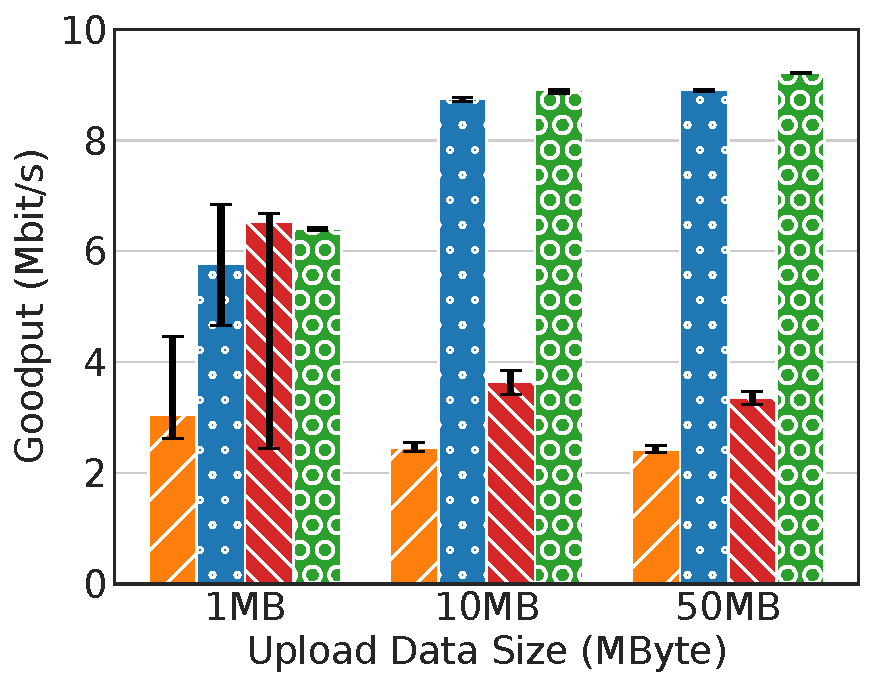
\includegraphics[width=\linewidth]{figures/fig5_baseline_loss1p.pdf}
	\caption{1\% loss.}
	\label{fig:baseline-bar:loss1p}
\end{subfigure}
\vspace{-0.2cm}
\caption{Median goodput for three upload data sizes with $0\%$ and $1\%$ loss on
Link 1. 20 trials. Error bars are 1st and 3rd quartiles.
With proxy assistance at $1\%$
loss, both QUIC and TCP match the performance of when there is no loss at all.
\vspace{-0.4cm}
}
\label{fig:baseline-bar}
\end{figure}

\begin{figure}[t]
\centering
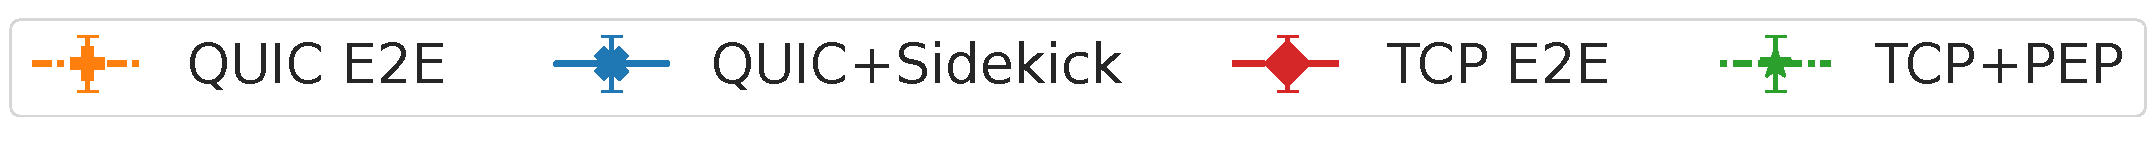
\includegraphics[width=\columnwidth]{figures/fig6_legend.pdf}
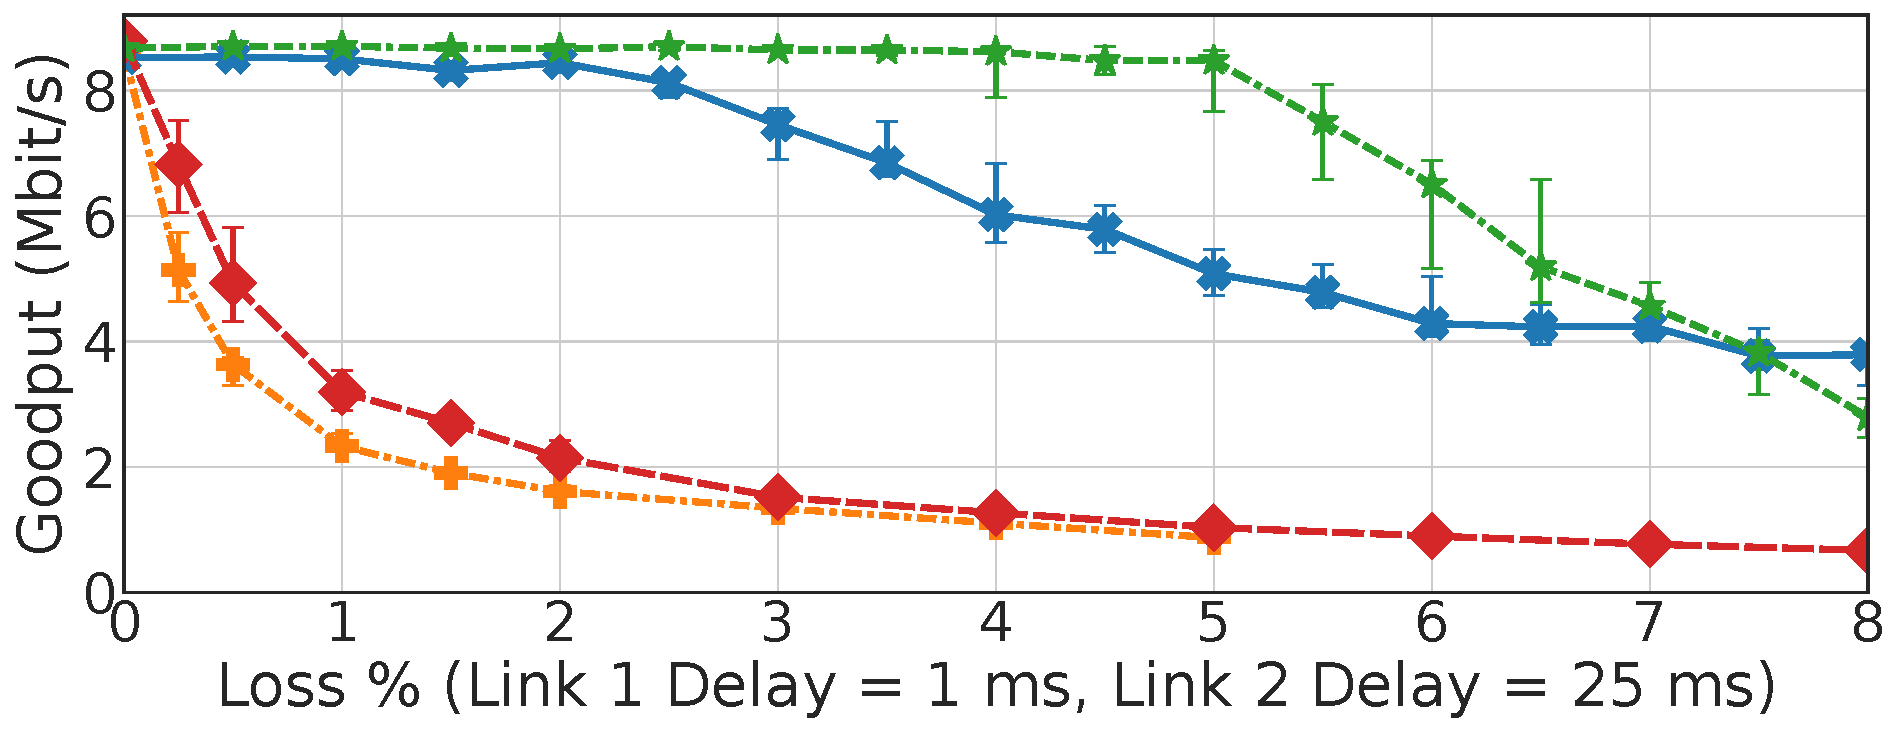
\includegraphics[width=\columnwidth]{figures/fig6_loss_bw100_10M_delay_25ms_1ms.pdf}
%\includegraphics[width=\columnwidth]{figures/loss_bw100_10M_delay_15ms_11ms.pdf}
\vspace{-0.4cm}
\caption{Connection-splitting PEP emulation as a function of near-segment
	loss rate. In this emulation experiment, QUIC+\Sys (running PACUBIC)
  performs similarly to TCP+PEP (each connection running CUBIC)
  and improves goodput compared with end-to-end protocols. The graph shows
  median goodput of a 10~MByte upload. QuACK interval is 30~ms, threshold
is 10. Error bars show IQR of 10 trials.
\vspace{-1cm}
}
\label{fig:loss-vs-tput}
\end{figure}

%\begin{figure}[t]
%\centering
%	\includegraphics[width=0.6\linewidth]{figures/multiflow_loss0p_legend.pdf}\\
%	\includegraphics[width=0.32\linewidth]{figures/quic_quack_60M_loss0p_delay0s_bw100.pdf}
%	\includegraphics[width=0.32\linewidth]{figures/quic_quack_60M_loss0p_delay5s_bw100.pdf}
%	\includegraphics[width=0.32\linewidth]{figures/quack_quic_60M_loss0p_delay5s_bw100.pdf}
%        \caption{Fairness evaluation of two concurrent QUIC flows in
%          Scenario \#1 (but without loss on the near path segment), one \sys-assisted and one end-to-end, in a purely
%          congestion-limited situation. The use of
%          \sys assistance doesn't affect 
%
%          Throughput of two concurrent flows in Scenario 1 (with $0\%$ and $1\%$
%loss on Link 1. Both flows converge to a steady-state throughput, whether the
%flows start at the same time (left) or at a 5 second delay (middle, right).}
%\label{fig:multiflow}
%\end{figure}

% \begin{figure*}
% \centering
% \includegraphics[width=\columnwidth]{figures/legend.pdf}\\
% \subfigure[QUIC, QUIC no delay]{
% 	\includegraphics[width=0.185\textwidth]{figures/quic_quic_60M_loss0p_delay0s.pdf}
% 	\label{fig:multiflow:a}}
% \subfigure[QUIC, QUIC 5s delay]{
% 	\includegraphics[width=0.185\textwidth]{figures/quic_quic_60M_loss0p_delay5s.pdf}
% 	\label{fig:multiflow:b}}
% \subfigure[QUIC, \sys no delay]{
% 	\includegraphics[width=0.185\textwidth]{figures/quic_quack_60M_loss0p_delay0s.pdf}
% 	\label{fig:multiflow:c}}
% % \subfigure[quack, quic no delay]{
% % 	\includegraphics[width=0.185\textwidth]{figures/quack_quic_60M_loss0p_delay0s.pdf}}
% \subfigure[QUIC, \sys 5s delay]{
% 	\includegraphics[width=0.185\textwidth]{figures/quic_quack_60M_loss0p_delay5s.pdf}
% 	\label{fig:multiflow:d}}
% \subfigure[\sys, QUIC 5s delay]{
% 	\includegraphics[width=0.185\textwidth]{figures/quack_quic_60M_loss0p_delay5s.pdf}
% 	\label{fig:multiflow:e}}
% % \label{fig:multiflow:quic-quack}
% % \end{figure*}

% % \begin{figure*}
% % \centering
% \subfigure[PEP, PEP no delay]{
% 	\includegraphics[width=0.185\textwidth]{figures/pep_pep_60M_loss1p_delay0s.pdf}
% 	\label{fig:multiflow:f}}
% \subfigure[PEP, PEP 5s delay]{
% 	\includegraphics[width=0.185\textwidth]{figures/pep_pep_60M_loss1p_delay5s.pdf}
% 	\label{fig:multiflow:g}}
% \subfigure[PEP, \sys no delay]{
% 	\includegraphics[width=0.185\textwidth]{figures/pep_quack_60M_loss1p_delay0s.pdf}
% 	\label{fig:multiflow:h}}
% % \subfigure[quack, pep no delay]{
% % 	\includegraphics[width=0.185\textwidth]{figures/quack_pep_60M_loss1p_delay0s.pdf}}
% \subfigure[PEP, \sys 5s delay]{
% 	\includegraphics[width=0.185\textwidth]{figures/pep_quack_60M_loss1p_delay5s.pdf}
% 	\label{fig:multiflow:i}}
% \subfigure[\sys, PEP 5s delay]{
% 	\includegraphics[width=0.185\textwidth]{figures/quack_pep_60M_loss1p_delay5s.pdf}
% 	\label{fig:multiflow:j}}
% \caption{Multiflow experiment with various combinations of QUIC end-to-end and QUIC+\sys at 0\% loss (a-e),
% and various combinations of TCP+PEP and QUIC+\sys at 1\% loss (f-j), demonstrating
% flow fairness. The delay indicates how long we started the second flow after the first flow.}
% \label{fig:multiflow}
% \end{figure*}
